\documentclass{beamer}
\usetheme[
  block=fill,
  background=light,
  titleformat=smallcaps,
  progressbar=frametitle,
]{metropolis}


% Beamer
\setbeamertemplate{frametitle}[default][center]

\makeatletter
\setbeamertemplate{title page}{
  \begin{minipage}[b][\paperheight]{\textwidth}
    \centering  % <-- Center here
    \ifx\inserttitlegraphic\@empty\else\usebeamertemplate*{title graphic}\fi
    \vfill%
    \ifx\inserttitle\@empty\else\usebeamertemplate*{title}\fi
    \ifx\insertsubtitle\@empty\else\usebeamertemplate*{subtitle}\fi
    \usebeamertemplate*{title separator}
    \ifx\beamer@shortauthor\@empty\else\usebeamertemplate*{author}\fi
    \ifx\insertdate\@empty\else\usebeamertemplate*{date}\fi
    \ifx\insertinstitute\@empty\else\usebeamertemplate*{institute}\fi
    \vfill
    \vspace*{1mm}
  \end{minipage}
}

\setbeamertemplate{title}{
%  \raggedright%  % <-- Comment here
  \linespread{1.0}%
  \inserttitle%
  \par%
  \vspace*{0.5em}
}
\setbeamertemplate{subtitle}{
%  \raggedright%  % <-- Comment here
  \insertsubtitle%
  \par%
  \vspace*{0.5em}
}
\makeatother

\title{\centering Deductive Parsing}
\subtitle{with an Unbounded Type Lexicon}
\author{K. Kogkalidis, M. Moortgat, R. Moot, G. Tziafas}
\date{August 2019}
\institute{SemSpace 2019}

\usepackage{tabularx}
\usepackage{booktabs}
\usepackage{multicol}
\usepackage{multirow}
\newcolumntype{m}{>{\hsize=.7\hsize}X}
\newcolumntype{s}{>{\hsize=.3\hsize}X}
\usepackage{tikz}
\usetikzlibrary{calc}
\usepackage{amsmath}
\usetikzlibrary{decorations.pathmorphing}
\usepackage{proof}
\usepackage{pifont}
\usepackage{qtree}[center]
\usepackage{forest}
\usetikzlibrary{arrows.meta}
\usepackage{mathtools}
\usepackage{pgf}
\usepackage{graphicx}


\begin{document}
\maketitle

\begin{frame}{Why Parsing?}
\begin{block}{Compositionality}
	Meaning of complex expression derived by constituent expressions and their  \alt<2>{\alert {means of interaction}}{means of interaction}.
\end{block}
\vfill 

\pause
\textbf{Syntax}
\begin{itemize}
	\item[] Algebra of sentence \alert{structure}
	\item[] Base for linguistically informed compositional semantics
\end{itemize}

\end{frame}

\begin{frame}{Why Deductive?}
	\begin{minipage}[t]{0.65\textwidth}
	\invisible<1>{
	\textbf{Type-Logical Grammars}
	\begin{itemize}
		\item[] Words $\rightarrow$ Logical Formulas
		\item[] Well-Formedness $\equiv$ Provability
	\end{itemize}}
	\vfill	
		
	\visible<3->{
	\textbf{Curry-Howard Correspondence}
	\begin{itemize}
		\item[] Logical Formulas $\leftrightarrow$ Typed Variables
		\item[] Proofs $\equiv$ Functional Programs
	\end{itemize}}
	
	\visible<4->{\textbf{Syntax-Semantics Interface}
	\begin{itemize}
		\item[] Syntactic Types $\to$ Semantic Spaces
		\item[] Derivations $\to$ Semantic Programs
	\end{itemize}
	}
	

\end{minipage}%
	\begin{minipage}[t]{0.35\textwidth}
		\begin{figure}
	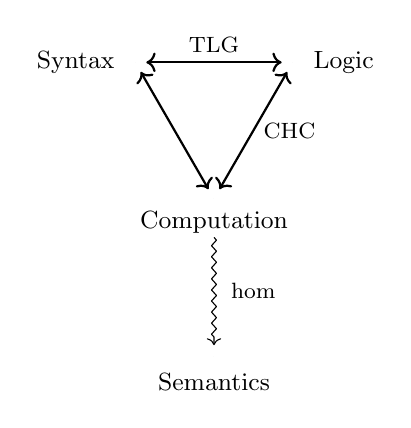
\begin{tikzpicture}[
		dot/.style={circle, inner sep=0pt, outer sep=4pt, minimum size=0pt, fill=black}
	]
		\visible<2->{\node[dot, label=right :{\small Logic}] (lo) at (0, 0) {};}
		\visible<1->{\node[dot, label=left:{\small Syntax}] (la) at ($(lo)+(0:-2)$) {};}
		\visible<3->{\node[dot, label={[yshift=-20pt]\small Computation}] (co) at ($(la)+(-60:2)$) {};}
		\visible<4->{\node[dot, label={[yshift=-20pt]\small Semantics}] (sem) at ($(co) + (0,-2)$) {};}		
				
		\visible<2->{\draw (lo) edge[<->, thick] node[midway, above] {\footnotesize TLG} (la);}
		\visible<3->{\draw (la) edge[<->, thick] (co);}
		\visible<3->{\draw (co) edge[<->,  thick] node[midway, right] {\footnotesize CHC} (lo);}
		
		\tikzset{decoration={snake,amplitude=.4mm,segment length=2mm,
                       post length=0mm,pre length=0mm}}
         \visible<4->{\draw [->, line join=round, decorate, decoration={	zigzag, segment length=4, amplitude=.9, post=lineto, post length=2pt}] ($(co.south) + (0, -.35)$) -> (sem);
		\node[label=above:{\footnotesize hom}] at (-0.5,-3.25) {};}
	\end{tikzpicture}
\end{figure}	
	\end{minipage}
\end{frame}

\begin{frame}{A Dependency-Decorated TLG}
\textbf{Lexicon}: Words $\rightarrow$ dependency-decorated MILL types \small{(\textit{\`{a} la ACG})}
\begin{itemize}
	\item[] Constants: \{ \textsc{np}, \textsc{s}, \textsc{pron} \dots \}
	\item[] Functions: \{ $\diamond^\text{su}\textsc{np}\rightarrow\textsc{s}$, $\diamond^\text{su}\textsc{np}\rightarrow\left(\diamond^\text{obj}\textsc{np}\rightarrow\textsc{s} \right)$, \dots \}
\end{itemize}


\[
\mathcal{T} := A \ | \ \diamond^d T_0 \ | \ T_1 \to T_2
\]
\vfill 

\pause 
\textbf{Parsing}: Proof Search
    \begin{align*}
    \begin{minipage}{0.5\textwidth}
		\[
	        \infer[\rightarrow E]{\Gamma, \Delta \vdash s\langle t \rangle: B}{
	            \Gamma \vdash s: A \rightarrow B
	            &
	            \Delta \vdash t: A
	        }
	    \]
	    \end{minipage}%
	    \begin{minipage}{0.5\textwidth}
	    \[
	        \infer[\rightarrow I]{\Gamma \vdash \lambda x.u : A \rightarrow B}{
	            \Gamma, x: A \vdash u: B
	        }
	    \]
    	\end{minipage}
    \end{align*}
\end{frame}

\begin{frame}{Parsing Framework}	
	
	\textbf{\alert{Parse State}}
	\begin{itemize}
		\item A logical judgement (premises \& conclusion)
		\item Word associations for (some) premise formulas
		\item A single element stack
	\end{itemize}
	
	\pause
	\textbf{\alert{Framework}}
	
	Given a parse state
	\begin{itemize}
		\item[1] Decide between introduction $\oplus$ elimination
		\item[2] Perform either
		\item[3] Update state(s) 
		\item[4] Repeat
	\end{itemize}		
\end{frame}


\begin{frame}{Ambiguities \footnotesize{(the bad kind)}}
\begin{center}
\small 
	$\mathcal{L}$ := \{``\textit{ducks}'': $\textsc{np}$, ``\textit{eat}'': $\diamond^\text{su}\textsc{np}\to\left(\diamond^\text{obj}\textsc{np}\to\textsc{s}\right)$, ``\textit{seeds}'': $\textsc{np}$\}
	
	``\textit{ducks eat seeds}'' $\vdash^{?}$ \textsc{s} 
\end{center}

\pause 
\begin{minipage}{0.45\textwidth}
	\footnotesize 
	\begin{forest}
	    for tree={
        l sep=5,
    	    parent anchor=south,
        child anchor=north,
        font=\sffamily,
	}
	[$\textsc{s}$
		[$\diamond^\text{obj}\textsc{np}\to\textsc{s}$
			[$\diamond^\text{su}\textsc{np}$
				[$\textsc{np}$
					[ducks]]
			]
			[$\diamond^\text{su}\textsc{np}\to\left(\diamond^\text{obj}\textsc{np}\to\textsc{s}\right)$
				[eat]]
		]
		[$\diamond^\text{obj}\textsc{np}$
			[$\textsc{np}$
				[seeds]
			]
		]
	]			
\end{forest}	
\center \texttt{(eat seeds) ducks} {\large\color{blue}\checkmark}
\end{minipage}%
\pause
\hfill
\begin{minipage}{0.45\textwidth}
\footnotesize
\begin{forest}
    for tree={
        l sep=5,
    	    parent anchor=south,
        child anchor=north,
        font=\sffamily,
}
	[$\textsc{s}$
		[$\diamond^\text{obj}\textsc{np}$
			[$\textsc{np}$
				[ducks]
			]
		]
		[$\diamond^\text{obj}\textsc{np}\to\textsc{s}$
			[$\diamond^\text{su}\textsc{np}\to\left(\diamond^\text{obj}\textsc{np}\to\textsc{s}\right)$
				[eat]]
			[$\diamond^\text{su}\textsc{np}$
				[$\textsc{np}$
					[seeds]]
			]
		]
	]			
\end{forest}	
\center \texttt{(eat ducks) seeds} {\large\color{red}\ding{55}}
\end{minipage}
\end{frame}

\begin{frame}{Resolving Ambiguities}
	\begin{block}{Key insight}
		Structure can be disambiguated by utilizing \alert{word} and \alert{position} information on top of \alert{types}.
	\end{block}
	\vfill
	
	\pause
	\textbf{Words (\& Position)}

	Contextualized embeddings from some LM
	\vfill
	
	\pause
	\textbf{Types}
	
	Type-level recursive GRU
	\begin{itemize}
		\item[] $\lceil A \rceil$ = $\overrightarrow{A}$
		\item[] $\lceil \diamond^d X \to Y \rceil$ = \textit{GRU}
			$ \left( \left[
				\overrightarrow{d}, \lceil X \rceil, \lceil Y \rceil 
			\right] \right) $
		
	\end{itemize}
	\vfill 
\end{frame}

\begin{frame}{Elimination $\sim$ \alt<3->{\alert{Binary Classification}}{?}}

\begin{block}{Problem}
Given a \textit{judgement}, decide between possible \textit{branchings}..

\pause 
.. given a sequence of \textit{word \& type pairs}, assign each item a \alert{\textit{binary label}}
\end{block}
\vfill

\pause
\textbf{Binary Sequence classification} \small{(Deep bi-GRU)}
\begin{itemize}
	\item[{
\includegraphics[scale=0.01]{duck.pdf}}] \textbf{Input}: Sequence of word \& type vectors \small{(conc.)}
	\item[{
\includegraphics[scale=0.01]{duck.pdf}}] \textbf{Output}: Sequence of binary labels
\end{itemize}	\vfill

\end{frame}

\begin{frame}{Proof Traversal}
    \small 
    \begin{minipage}{0.3\textheight}
        \infer[]{\text{ducks}, \text{eat}, \text{seeds} \vdash \textsc{s}}{
            \infer[\rightarrow E]{\text{eat}, \text{seeds} \vdash \textsc{np}\to\textsc{s}}{
                \infer[Ax.]{\text{eat} \vdash \textsc{np}\to\textsc{np}\to\textsc{s}}{}
                &
                {\color<6->{blue}\infer[Ax.]{\text{seeds} \vdash \textsc{np}}{}}
            }
            &
            {\color<4->{red}\infer[Ax.]{\text{ducks} \vdash \textsc{np}}{}}
        }
    \end{minipage}
    \begin{minipage}{0.6\textheight}
    \begin{figure}
    \centering
    \begin{tikzpicture}
        \small 
        
    	\node[rectangle, inner sep=0pt, minimum width=120pt, minimum height=20pt] (ducks) at (0, -1.5) {\alt<5->{}{{\color<4->{red}$
    	\left( \overrightarrow{\text{ducks}}; \lceil \textsc{np} \rceil \right) $}, } 
    	$\left( \overrightarrow{\text{eat}}; \lceil \textsc{np}\to\textsc{np}\to\textsc{s} \rceil \right)$,
    	 {\color<6->{blue}{
    	 $\left( \overrightarrow{\text{seeds}}; \lceil \textsc{np} \rceil \right)$ $\vdash$}} \alt<5->{$\lceil \textsc{np}\to\textsc{s} \rceil $}{$\lceil \textsc{s} \rceil$}};

    	\node[draw=white, rectangle, minimum width=240pt, minimum height=20pt, ultra thick, fill=black] (bb) at (0, 0) {\color{white}{Deep bi-GRU}};
    	
    	\pause
    	\node[rectangle, inner sep=0pt, minimum width=120pt, minimum height=20pt] (ducks) at (0, -1.5) {};
    	\draw ($(ducks.north) + (0, 0)$) edge[->, ultra thick] node[above] {} ($(bb.south) + (0, 0)$);
    	
    	\pause
    	\invisible<5->{\node[rectangle, inner sep=0pt, minimum width=120pt, minimum height=20pt] (ducktype) at (-2.5, 1.5) {{\color<4->{red}\textsc{1}}};
    	\draw ($(ducktype.south) + (0, 0)$) edge[<-, ultra thick] node[above] {} ($(bb.north) + (-2.5, 0)$);}
    	\invisible<5>{\node[rectangle, inner sep=0pt, minimum width=120pt, minimum height=20pt] (eattype) at (-0.8, 1.5) {\textsc{0}};}
    	\invisible<5>{\draw ($(eattype.south) + (0, 0)$) edge[<-, ultra thick] node[above] {} ($(bb.north) + (-0.8, 0)$);}
    	\alt<6->{
    	\node[rectangle, inner sep=0pt, minimum width=120pt, minimum height=20pt] (fishtype) at (2.5, 1.5) {{\color<6->{blue}{\textsc{1}}}};
    	}{
    	\invisible<5>{\node[rectangle, inner sep=0pt, minimum width=120pt, minimum height=20pt] (fishtype) at (2.5, 1.5) {\textsc{0}};}}
    	\invisible<5>{\draw ($(fishtype.south) + (0, 0)$) edge[<-, ultra thick] node[above] {} ($(bb.north) + (2.5, 0)$);}

    \end{tikzpicture}
    \end{figure}
    \end{minipage} 
    \vfill 
   
	\only<8>{
	\[
	\begin{rcases*}
		\text{Training sample} \ &: \ \text{Junction point} \\
		\text{Sentence} \ 	&: \ \text{N independent samples} \\
	\end{rcases*}  \text{\alert{Massive Parallelism}}
	\]
    }
\end{frame}

\begin{frame}{..but is it working?}
\textbf{Some Concessions}
\begin{itemize}
	\item[] Up to 2nd order types
	\item[] No conjunctions
	\item[] Gold types as input
\end{itemize}

\pause
\textbf{Table with Numbers}

\quad\quad\begin{tabularx}{0.65\textwidth}{ms}
	\textit{Input} & \textit{Accuracy} \\
	\hline
	Types \& Words \& Goal & \textbf{97.2}\\
	Types \& Words & 95.3\\
	Types only & 94.2 \\
	Words only & 87.7 \\
\end{tabularx}
\end{frame}

\begin{frame}{Conclusion \& Future}
\begin{minipage}[t]{0.6\textwidth}
	\textbf{Neural TLG Parsing}
	\begin{itemize}
	\item[{
\includegraphics[scale=0.01]{duck.pdf}}] Fast \& Efficient
	\item[{
\includegraphics[scale=0.01]{duck.pdf}}] Accurate
	\item[{
\includegraphics[scale=0.01]{duck.pdf}}] Formally grounded
	\item[{
\includegraphics[scale=0.01]{duck.pdf}}] Ideal for semantic tasks	
	\end{itemize}
	\end{minipage}
	\vfill 
	
	\begin{minipage}[t]{0.8\textwidth}
	\textbf{\color{purple}{\# todo}}
	\begin{itemize}
	\item[{
\includegraphics[scale=0.01]{duck.pdf}}] End-to-end integration \& evaluation
	\item[{
\includegraphics[scale=0.01]{duck.pdf}}] Higher-order structures
	\item[{
\includegraphics[scale=0.01]{duck.pdf}}] Other approaches (.. Shift-Reduce, ProofNets?)
		\pause
	\item[{
\includegraphics[scale=0.01]{duck.pdf}}] \alert{Thank audience}
	\end{itemize}	
	\end{minipage}
\end{frame}


\end{document}